% Provenance (never printed): see sources/outline_sources.md (Year 3:
% fractionation and Rayleigh distillation in the water cycle;
% palaeothermometry; carbon and sulfur isotopes). Brief:
% sources/book5/BRIEFS.md, ch. 14. Curves from figdata/bachelor-3/
% rayleigh_distillation.py, lr04_d18o.py, carbon_mass_balance.py. Exercise
% and problem values in the Book 5 scratch calculator calc/ch14.py. Dome Ilse,
% its traverse and the marine core are invented.
\chapter{Geochemie van stabiele isotopen}\label{ch:b3:stable-isotopes}

Sneeuw die op de hoge koepels van de Oost-Antarctische ijskap valt, behoort
tot het lichtste water op Aarde. Elk van zijn moleculen verliet de oceaan als waterdamp, en
onderweg naar het binnenland verloor de lucht het grootste deel van haar water als sneeuw, de zware moleculen
eerst. Wat bij aankomst overblijft, hangt af van hoeveel er verloren ging, en dat hangt af van
hoe koud de lucht is geworden. Een ijskolom is daarom een thermometer, een schelp
van calciet een andere, en de koolstof van kalksteen een grootboek van wat de
biosfeer begroef. Dit hoofdstuk leidt de wetten af die achter deze archieven schuilen en
leest ze uit.

\begin{recall}
De $\delta$-waarde, de fractioneringsfactor $\alpha$ en de evenwichts- en
kinetische isotopeneffecten staan in de universitaire delen van de scheikundeboeken. De
referentiestandaarden VSMOW en VPDB en de meteorische waterlijn staan in
Boek~4, in het hoofdstuk over isotopengeochemie; de Rayleighfractioneringswet
voor sporenelementen in het hoofdstuk over magmatische
differentiatie; klimaatproxy's, het ijsvolume-effect en de Mg/Ca-
thermometer in het hoofdstuk over klimaatarchieven en proxy's; de
Paleoceen-Eoceen Thermisch Maximum in het hoofdstuk over het klimaat in de geologische
tijd; de Grote Oxidatiegebeurtenis in het hoofdstuk over de Precambrische Aarde.
Fotosynthese en bacteriële sulfaatreductie staan in de biologieboeken.
\end{recall}

\section{Fractionering tussen twee fasen}\label{sec:b3:stable-isotopes:fractionation}

Voor twee fasen A en B in isotopisch evenwicht is $\alpha_{A-B} = R_A/R_B =
(1000 + \delta_A)/(1000 + \delta_B)$, met de verhoudingen $R$ van het zware tot het
lichte isotoop. Waterdamp en vloeibaar water hebben $\alpha = 1.0098$ voor zuurstof-18
en $1.084$ voor deuterium bij \qty{20}{\celsius}, $1.0117$ en $1.111$ bij
\qty{0}{\celsius}; ijs en water bij \qty{0}{\celsius}, $1.0035$ en $1.0208$.
De zwaardere fase is altijd de meest gecondenseerde, en de fractionering
neemt toe naarmate de temperatuur daalt.
% ledger: kc98:alpha, kc98:standards

\begin{definition}[Isotopenverschil]\label{def:b3:stable-isotopes:big-delta}
Het \emph{isotopenverschil}\index{isotopenverschil (hoofdletter delta)}
tussen twee fasen is $\Delta_{A-B} = \delta_A - \delta_B$, in promille.
\end{definition}

\begin{proposition}[Het isotopenverschil en de fractioneringsfactor]
\label{prop:b3:stable-isotopes:big-delta}
Voor $\alpha$ dicht bij 1 en kleine $\delta$-waarden,
\[
\Delta_{A-B} \approx 1000\ln\alpha_{A-B} \approx 1000(\alpha_{A-B} - 1).
\]
\end{proposition}

\begin{proof}
$1000\ln\alpha = 1000\ln(1 + \delta_A/1000) - 1000\ln(1 + \delta_B/1000)$, en
$1000\ln(1 + x/1000) = x - x^2/2000 + \dots$, dus $1000\ln\alpha = \delta_A -
\delta_B - (\delta_A^2 - \delta_B^2)/2000 + \dots$. Tot slot $\ln\alpha \approx
\alpha - 1$ voor $\alpha$ dicht bij 1.
\end{proof}

De fout is $(\delta_A^2 - \delta_B^2)/2000$: een fractie van een promille bij de
waarden van de oceaan, bijna een promille tussen de oceaan en de lichte sneeuw van
poolijs.
De grootheid $1000\ln\alpha$ is de grootheid die de theorie met de temperatuur verbindt: zij
varieert bijna als $1/T^2$ bij hoge temperatuur en als $1/T$ bij lage temperatuur,
en ijkingen worden in die vorm geschreven. Voor ijs en waterdamp bijvoorbeeld,
\[
\ln\alpha^{18}_{\mathrm{ice-v}} = \frac{11.839}{T} - 0.028224, \qquad
\ln\alpha^{\mathrm D}_{\mathrm{ice-v}} = \frac{16288}{T^2} - 0.0934,
\]
met $T$ in kelvin.
% ledger: gkinis14:alpha-ice, kc98:standards

\begin{definition}[Massa-afhankelijke en massa-onafhankelijke fractionering]\label{def:b3:stable-isotopes:mif}
Een element met drie isotopen of meer heeft een \emph{massa-afhankelijke
fractionering}\index{massa-afhankelijke fractionering} wanneer de fractioneringen van
zijn isotoopverhoudingen zich verhouden als hun massaverschillen, zoals bepaald door de
massa's; anders heeft het een \emph{massa-onafhankelijke
fractionering}\index{massa-onafhankelijke fractionering}, gemeten door de afwijking
van de massa-afhankelijke lijn, zoals $\Delta^{33}\mathrm S = \delta^{33}\mathrm S
- 0.515\,\delta^{34}\mathrm S$.
\end{definition}

Voor zuurstof is de fractionering van $^{17}\mathrm O/^{16}\mathrm O$ ongeveer 0.52 keer die
van $^{18}\mathrm O/^{16}\mathrm O$, dicht bij de verhouding van de massaverschillen, 1 tot 2;
voor zwavel, $\delta^{33}\mathrm S = 0.515\,\delta^{34}\mathrm S$. \omterm{def:b3:stable-isotopes:mif}{Massa-onafhankelijke
fractionering} is zeldzaam: zij wordt aangetroffen in meteorieten, in stratosferisch ozon en
in Archeïsche zwavel.
% ledger: white13c9:mdf, white13c9:s-mif

\section{Rayleighdestillatie in de watercyclus}\label{sec:b3:stable-isotopes:rayleigh}

Een luchtmassa die afkoelt, vormt wolkendruppels of sneeuwkristallen, die vallen en
de luchtmassa verlaten. Elk condensaat is rijker aan de zware isotopen dan de waterdamp, zodat de
resterende waterdamp wordt lichter, en het volgende condensaat, in evenwicht ermee, is
eveneens lichter.

\begin{proposition}[Rayleighdestillatie]\label{prop:b3:stable-isotopes:rayleigh-distillation}
Beschouw een reservoir van waterdamp dat zijn water verliest door condensaten, elk verwijderd zodra
het in evenwicht met de waterdamp is gevormd. Als $f$ de fractie van de
resterende waterdamp is en $\alpha$ de fractioneringsfactor condensaat-waterdamp, dan
voldoet de verhouding van de waterdamp aan $\mathrm d\ln R_v = (\alpha - 1)\,\mathrm d\ln f$. Voor
een constante $\alpha$ is dit de \emph{Rayleigh
destillatie}\index{Rayleighdestillatie}:
\[
\frac{R_v}{R_{v,0}} = f^{\,\alpha - 1}, \qquad
\delta_v = (1000 + \delta_{v,0})\,f^{\,\alpha - 1} - 1000,
\]
en het bij $f$ gevormde condensaat heeft $\delta_c = \alpha(1000 + \delta_v) - 1000$.
\end{proposition}

\begin{proof}
Laat $N$ het aantal moleculen waterdamp zijn (bijna allemaal licht) en $N R_v$
het aantal zware. Het verwijderen van $\mathrm dN < 0$ moleculen condensaat
verwijdert $\alpha R_v\,\mathrm dN$ zware: $\mathrm d(NR_v) = \alpha
R_v\,\mathrm dN$. Hieruit volgt $N\,\mathrm dR_v = (\alpha - 1)R_v\,\mathrm dN$, wat de
differentiële wet met $f = N/N_0$ is. Bij een constante $\alpha$ integreert deze tot
de machtswet.
\end{proof}

Als $\alpha$ van de temperatuur afhangt, geldt langs het traject $\ln(R_v/R_{v,0}) = \int(\alpha - 1)\,
\mathrm d\ln f$. Voor een luchtmassa die bij constante druk afkoelt,
wordt de waterdamp die zij kan bevatten bepaald door de verzadigingsdruk, dus $f =
e_s(T)/e_s(T_0)$, wat de sublimatiecurve van ijs geeft onder
\qty{0}{\celsius}. De onderstaande figuur integreert de wet voor een luchtmassa waarvan de
waterdamp begint op \qty{0}{\celsius} met een veronderstelde $\delta^{18}\mathrm O = -20$
en $\delta\mathrm D = \qty{-150}{\permil}$. Echte waterdamp boven de oceaan is
lichter dan evenwicht met zeewater zou geven, ongeveer $-13$ in plaats van
\qty{-9}{\permil} voor zuurstof-18, omdat verdamping deels kinetisch is.
% ledger: iapws:melt-subl, gkinis14:alpha-ice, white13c9:rayleigh

\begin{definition}[Deuteriumoverschot]\label{def:b3:stable-isotopes:d-excess}
Het \emph{deuteriumoverschot}\index{deuteriumoverschot} van een watermonster is $d =
\delta\mathrm D - 8\,\delta^{18}\mathrm O$, in promille.
\end{definition}

Neerslag van de continenten op het Noordelijk Halfrond ligt op de lijn
$\delta\mathrm D = 8.0\,\delta^{18}\mathrm O + 10$: het \omterm{def:b3:stable-isotopes:d-excess}{deuteriumoverschot} ervan is ongeveer
\qty{10}{\permil}. De helling 8 ligt dicht bij de verhouding van de evenwichtsfractioneringen
van de twee isotopen bij condensatie. Het overschot van 10, niet 0,
legt de kinetische verdamping vanuit de oceaan vast, en het overschot van een monster
meet hoe ver van evenwicht het water ervan verdampte.
% ledger: dansgaard64:effects, kc98:mwl

\begin{omfigure}
\begin{tikzpicture}
\begin{groupplot}[group style={group size=2 by 1, horizontal sep=1.6cm},
  omrecord, width=0.47\linewidth, height=0.42\linewidth, title style={font=\small},
  tick label style={font=\scriptsize}, label style={font=\small},
  legend style={font=\scriptsize, legend cell align=left}]
\nextgroupplot[title={(a) langs het afkoelingstraject},
  xlabel={condensatietemperatuur (\unit{\celsius})}, ylabel={$\delta^{18}\mathrm O$ (\unit{\permil})},
  xmin=-55, xmax=0, ymin=-130, ymax=0, x dir=reverse,
  legend style={at={(0.03,0.03)}, anchor=south west}]
% computed in figdata/bachelor-3/rayleigh_distillation.py
\addplot[omDef, thick, densely dashed] table[x=t, y=d18v] {figdata/out/bachelor-3-rayleigh_distillation-curve.dat};
\addlegendentry{waterdamp}
\addplot[omDef, thick] table[x=t, y=d18s] {figdata/out/bachelor-3-rayleigh_distillation-curve.dat};
\addlegendentry{sneeuw}
\addplot[red!70!black, only marks, mark=*, mark size=1.6pt] table[x=t, y=d18s] {figdata/out/bachelor-3-rayleigh_distillation-stations.dat};
\addlegendentry{stations}
\nextgroupplot[title={(b) de sneeuw in het $\delta\mathrm D$--$\delta^{18}\mathrm O$-diagram},
  xlabel={$\delta^{18}\mathrm O$ (\unit{\permil})}, ylabel={$\delta\mathrm D$ (\unit{\permil})},
  xmin=-110, xmax=0, ymin=-700, ymax=0,
  legend style={at={(0.97,0.03)}, anchor=south east}]
\addplot[omDef, thick] table[x=d18s, y=dDs] {figdata/out/bachelor-3-rayleigh_distillation-curve.dat};
\addlegendentry{modelsneeuw}
\addplot[black, densely dotted, domain=-110:0, samples=2] {8*x + 10};
\addlegendentry{$\delta\mathrm D = 8\,\delta^{18}\mathrm O + 10$}
\addplot[red!70!black, only marks, mark=*, mark size=1.6pt, forget plot] table[x=d18s, y=dDs] {figdata/out/bachelor-3-rayleigh_distillation-stations.dat};
\end{groupplot}
\end{tikzpicture}

\par\smallskip{\small \omterm{prop:b3:stable-isotopes:rayleigh-distillation}{Rayleighdestillatie} van een luchtmassa die bij constante
druk afkoelt vanaf \qty{0}{\celsius}, met de ijs-waterdamp-fractioneringsfactoren
en de resterende fractie waterdamp, afgelezen uit de sublimatiecurve van ijs. (a) De
waterdamp (gestreept) en de sneeuw (doorgetrokken) worden steeds sneller lichter; de stippen zijn de
drie stations van het weekendprobleem. (b) De modelsneeuw blijft dicht bij de
meteorische waterlijn tot ongeveer \qty{-30}{\permil} voor zuurstof-18 en stijgt dan
erboven.}\label{fig:b3:stable-isotopes:rayleigh}
\end{omfigure}
% ledger: kc98:mwl


\begin{definition}[Temperatuur-, hoeveelheids- en continentaal effect]\label{def:b3:stable-isotopes:effects}
Het \emph{temperatuureffect}\index{temperatuureffect (isotopisch)} is de
afname van $\delta^{18}\mathrm O$ en $\delta\mathrm D$ van neerslag met de
lokale temperatuur. Het \emph{hoeveelheidseffect}\index{hoeveelheidseffect} is hun
afname met de hoeveelheid regen, in de tropen. Het \emph{continentaal
effect}\index{continentaal effect} is hun afname landinwaarts, bij een gegeven
temperatuur.
\end{definition}

Alle drie zijn \omterm{prop:b3:stable-isotopes:rayleigh-distillation}{Rayleighdestillatie} gezien vanaf de grond. Op hoge breedten
domineert het \omterm{def:b3:stable-isotopes:effects}{temperatuureffect}: de jaargemiddelden van Groenland en
de Noord-Atlantische stations volgen $\delta^{18}\mathrm O = 0.69\,t - 13.6$ en $\delta\mathrm D =
5.6\,t - 100$ (in promille, met $t$ de gemiddelde jaarlijkse oppervlaktetemperatuur in
\unit{\celsius}). In de tropen domineert het \omterm{def:b3:stable-isotopes:effects}{hoeveelheidseffect}: op één oceaaneiland
verliest maandelijkse regen ongeveer \qty{1.6}{\permil} zuurstof-18 voor elke
\qty{100}{mm} extra regen. Het eenvoudige model van de figuur hierboven geeft een steilere
helling, ongeveer \qty{1.6}{\permil} per graad condensatietemperatuur. De
hellingen zijn niet rechtstreeks vergelijkbaar: het oppervlak van een ijskap is kouder
dan de lucht waar de sneeuw vormt, en het model negeert de menging van luchtmassa's
en de kinetische effecten van sneeuwvorming, dus de helling ten opzichte van de
oppervlaktetemperatuur is gekalibreerd, niet berekend.
% ledger: dansgaard64:effects

\section{Paleothermometrie}\label{sec:b3:stable-isotopes:palaeothermometry}

\begin{definition}[Paleothermometrie, paleotemperatuurvergelijking]
\label{def:b3:stable-isotopes:palaeothermometry}
\emph{Paleothermometrie}\index{paleothermometrie} is het meten van vroegere
temperaturen uit de samenstelling van materialen die toen zijn gevormd. Een
\emph{paleotemperatuurvergelijking}\index{paleotemperatuurvergelijking} is een
gekalibreerde relatie tussen de vormingstemperatuur van een mineraal en de
fractionering met het water waaruit het groeide.
\end{definition}

Voor calciet dat langzaam uit water neerslaat, geeft één kalibratie
\[
1000\ln\alpha_{\mathrm{calcite-water}} = 18.03\,\frac{10^3}{T} - 32.42,
\]
met beide $\delta$-waarden op de VSMOW-schaal. Carbonaten worden gerapporteerd op de
VPDB-schaal, omgerekend met $\delta^{18}\mathrm O_{\mathrm{VPDB}} =
0.97001\,\delta^{18}\mathrm O_{\mathrm{VSMOW}} - 29.99$. Nabij \qty{5}{\celsius} daalt de
fractionering met ongeveer \qty{0.23}{\permil} per graad opwarming.
% ledger: isogeochem:ko97

\begin{method}[Een carbonaat-paleotemperatuur]\label{met:b3:stable-isotopes:palaeotemperature}
\begin{enumerate}
\item reken de $\delta^{18}\mathrm O$ van het calciet om van VPDB naar VSMOW;
\item schat de $\delta^{18}\mathrm O$ van het water waaruit de schelp groeide, op
VSMOW, waarbij de huidige waarde wordt gecorrigeerd voor het ijsvolume van die tijd;
\item bereken $1000\ln\alpha = 1000\ln[(1000 + \delta_c)/(1000 + \delta_w)]$;
\item keer de kalibratie om: $T = 18.03\times10^3/(1000\ln\alpha + 32.42)$.
\end{enumerate}
\end{method}

De tweede stap is de moeilijke. Tijdens een glaciatie slaan de ijskappen
licht water op, en wordt de oceaan zwaarder. Elke meter zeeniveau komt overeen
met ongeveer \qty{0.011}{\permil} van de $\delta^{18}\mathrm O$ van de oceaan; het laatste glaciale
maximum verlaagde het zeeniveau met ongeveer \qty{125}{m}, waardoor de oceaan ongeveer
\qty{1.4}{\permil} zwaarder werd. Organismen voegen hun eigen afwijkingen toe, de vitale
effecten, en een schelp kan na begraving zuurstof uitwisselen met poriewater.
% ledger: white13c9:ice-volume

\begin{omfigure}
\begin{tikzpicture}
\begin{axis}[omrecord, width=0.8\linewidth, height=0.32\linewidth, clip=false,
  xlabel={ouderdom (\unit{\ka})}, ylabel={benthische $\delta^{18}\mathrm O$ (\unit{\permil})},
  xmin=0, xmax=800, ymin=2.8, ymax=5.4, y dir=reverse,
  xtick={0,100,200,300,400,500,600,700,800},
  tick label style={font=\scriptsize}, label style={font=\small}]
% computed in figdata/bachelor-3/lr04_d18o.py from data/derived/lr04.csv
\addplot[omDef, thin] table[x=age_ka, y=d18O] {figdata/out/bachelor-3-lr04_d18o-stack.dat};
\draw[densely dotted] (axis cs:0,3.25) -- (axis cs:830,3.25);
\draw[densely dotted] (axis cs:20,5.02) -- (axis cs:830,5.02);
\draw[red!70!black, thick, |-|] (axis cs:830,3.25) -- node[right, font=\scriptsize, align=left] {ijsvolume\\\qty{1.4}{\permil}} (axis cs:830,4.625);
\draw[black, thick, |-|] (axis cs:830,4.625) -- node[right, font=\scriptsize] {afkoeling} (axis cs:830,5.02);
\end{axis}
\end{tikzpicture}

\par\smallskip{\small De globale stapel van benthische foraminiferen $\delta^{18}\mathrm O$
over de laatste \qty{800}{\ka}, de as omgekeerd zodat koude glaciale tijden
laag liggen. Van het heden (\qty{3.25}{\permil}) tot het laatste glaciale maximum
(\qty{5.02}{\permil}), ongeveer \qty{1.4}{\permil} van de verandering is het
ijsvolume (rode balk, rechts); de rest is een afkoeling van het diepe water (zwarte
balk).}\label{fig:b3:stable-isotopes:lr04}
\end{omfigure}
% ledger: data:lr04, white13c9:ice-volume

\begin{definition}[Geklonterde isotopen (clumped isotopes)]\label{def:b3:stable-isotopes:clumped}
\emph{Clumped isotopes}\index{clumped isotopes} zijn moleculen of groepen die
twee zware isotopen bevatten die aan elkaar gebonden zijn. In carbonaten is $\Delta_{47}$
het overschot, in promille, van de overvloed van $^{13}\mathrm C^{18}\mathrm O^{16}\mathrm O_2$
groepen, gemeten als kooldioxide met massa 47, ten opzichte van een willekeurige verdeling van de
isotopen.
\end{definition}

De zware isotopen binden zich iets vaker aan elkaar dan de kans zou doen verwachten,
en des te vaker naarmate het kristal kouder is. Het overschot hangt alleen af van de
temperatuur tijdens de groei, niet van de samenstelling van het water: één verenigde
kalibratie is $\Delta_{47} = 0.0391\times10^6/T^2 + 0.154$ (in promille, $T$
in kelvin) van 0.5 tot \qty{1100}{\celsius}. Samen gemeten met
$\delta^{18}\mathrm O$ levert dit zowel de temperatuur als de samenstelling van het
water op. De gevoeligheid is klein, ongeveer \qty{0.003}{\permil} per graad nabij
\qty{20}{\celsius}, wat lange metingen vereist.
% ledger: isogeochem:d47

\section{Koolstofisotopen}\label{sec:b3:stable-isotopes:carbon}

Fotosynthese fractioneert koolstof kinetisch. De diffusie van
kooldioxide in een blad kost ongeveer \qty{-4.4}{\permil}, het enzym RuBisCO
\qty{-29.4}{\permil}; planten van de gewone C3-route eindigen \num{20} tot
\qty{30}{\permil} lichter dan de lucht, en gemiddeld ongeveer
\qty{-27}{\permil}, die van de C4-route ongeveer \qty{-13}{\permil}. Organische
koolstof is licht, en de anorganische koolstof waaruit ze wordt gemaakt wordt zwaarder.
% ledger: white13c9:photosynthesis, white:d13c

\begin{definition}[Begravingsfractie van organische koolstof]\label{def:b3:stable-isotopes:forg}
De \emph{begravingsfractie van organische koolstof}\index{begravingsfractie van organische koolstof}
$f_{\mathrm{org}}$ is het deel van de koolstof die de oceaan en atmosfeer verlaat en
begraven wordt als organisch materiaal in plaats van als carbonaat.
\end{definition}

\begin{proposition}[Massabalans van koolstofisotopen]\label{prop:b3:stable-isotopes:forg}
In de stationaire toestand, met instroom van samenstelling $\delta_{\mathrm{in}}$ en begraving van
carbonaat $\delta_{\mathrm{carb}}$ en organische koolstof $\delta_{\mathrm{org}} =
\delta_{\mathrm{carb}} + \Delta_B$, de
\emph{massabalans van koolstofisotopen}\index{massabalans van koolstofisotopen} is
\[
\delta_{\mathrm{in}} = f_{\mathrm{org}}\,\delta_{\mathrm{org}} + (1 - f_{\mathrm{org}})\,
\delta_{\mathrm{carb}}, \qquad f_{\mathrm{org}} = \frac{\delta_{\mathrm{in}} -
\delta_{\mathrm{carb}}}{\Delta_B}.
\]
\end{proposition}

\begin{proof}
In de stationaire toestand is de koolstof die binnenkomt gelijk aan de koolstof die begraven
wordt, en dat geldt ook voor koolstof-13; met $\delta$-waarden is de balans van koolstof-13 een massagewogen
gemiddelde van de $\delta$-waarden, in de benadering van
\cref{prop:b3:stable-isotopes:big-delta}. Substitueer $\delta_{\mathrm{org}} =
\delta_{\mathrm{carb}} + \Delta_B$ en los op, dan volgt $f_{\mathrm{org}}$.
\end{proof}

De instroom, van vulkanen en de verwering van oude carbonaten en organisch materiaal, wordt
geschat op ongeveer \qty{-5}{\permil}, de waarde van de mantel; $\Delta_B$ is
tussen $-32$ en \qty{-25}{\permil} gebleven; en carbonaten hebben
in het grootste deel van de aardgeschiedenis een $\delta^{13}\mathrm C$ van rond 0 gehad,
binnen ongeveer \qty{1}{\permil}. De balans geeft dan de klassieke $f_{\mathrm{org}} \approx
0.2$: een vijfde van de koolstof wordt als organisch materiaal begraven, en daarmee
blijft de zuurstof die fotosynthese vrijmaakte in de lucht. Recent onderzoek stelt dat
$f_{\mathrm{org}}$ meer varieerde dan deze constantie doet vermoeden.
% ledger: planavsky22:forg

\begin{definition}[Koolstofisotopenexcursie]\label{def:b3:stable-isotopes:cie}
Een \emph{koolstofisotopenexcursie}\index{koolstofisotopenexcursie} is een
geologisch korte verschuiving van de $\delta^{13}\mathrm C$ van carbonaten en organisch
materiaal over de hele wereld, gevolgd door een terugkeer, zoals vastgelegd in sedimentaire profielen.
\end{definition}

\begin{proposition}[Massa van een excursie]\label{prop:b3:stable-isotopes:cie-mass}
Koolstof met samenstelling $\delta_s$ en massa $m$, gemengd in een uitwisselbaar
reservoir met massa $M$ en samenstelling $\delta_0$, verschuift het met $\Delta$ wanneer
\[
m = M\,\frac{\Delta}{\delta_s - \delta_0 - \Delta}.
\]
\end{proposition}

\begin{proof}
Het mengsel heeft $(M + m)(\delta_0 + \Delta) = M\delta_0 + m\delta_s$, lineair in
$m$.
\end{proof}

Bij het begin van het Paleoceen--Eoceen Thermisch Maximum, tussen 55.5 en
\qty{56.3}{\Ma} daalde de koolstof van de oceaan en de atmosfeer met 2.5 tot
\qty{4.0}{\permil} in minder dan \qty{60}{kyr}. De benodigde koolstof bedraagt ongeveer
2000 tot \qty{3500}{Gt} als het methaan was met \qty{-60}{\permil}, 6000 tot
\qty{12000}{Gt} als het organische koolstof was met \qty{-25}{\permil}: hoe lichter de
bron, hoe minder koolstof nodig is. Achterwaarts gelezen met de propositie
en $\delta_0 = 0$, impliceren deze schattingen een uitwisselbaar reservoir van \num{46000}
tot \qty{63000}{Gt} koolstof.
% ledger: dickens11:petm

\begin{omfigure}
\begin{tikzpicture}
\begin{groupplot}[group style={group size=2 by 1, horizontal sep=1.7cm},
  omrecord, width=0.47\linewidth, height=0.4\linewidth, title style={font=\small},
  tick label style={font=\scriptsize}, label style={font=\small},
  legend style={font=\scriptsize, legend cell align=left}]
\nextgroupplot[title={(a) stationaire toestand, $\delta_{\mathrm{in}} = \qty{-5}{\permil}$},
  xlabel={$f_{\mathrm{org}}$}, ylabel={$\delta^{13}\mathrm C_{\mathrm{carb}}$ (\unit{\permil})},
  xmin=0, xmax=0.4, ymin=-6, ymax=8, xtick={0,0.1,0.2,0.3,0.4}, xticklabels={0,0.1,0.2,0.3,0.4},
  legend style={at={(0.03,0.97)}, anchor=north west}]
% computed in figdata/bachelor-3/carbon_mass_balance.py
\addplot[omDef, thick] table[x=f, y=dcarb25] {figdata/out/bachelor-3-carbon_mass_balance-forg.dat};
\addlegendentry{$\Delta_B = \qty{-25}{\permil}$}
\addplot[red!70!black, thick] table[x=f, y=dcarb30] {figdata/out/bachelor-3-carbon_mass_balance-forg.dat};
\addlegendentry{$\Delta_B = \qty{-30}{\permil}$}
\nextgroupplot[title={(b) koolstof voor een excursie},
  xlabel={$\delta^{13}\mathrm C$ van de bron (\unit{\permil})}, ylabel={toegevoegde koolstof (\unit{Gt})},
  xmin=-70, xmax=-20, ymin=0, ymax=14000, scaled y ticks=false,
  ytick={0,4000,8000,12000}, yticklabels={0,4000,8000,12000},
  legend style={at={(0.03,0.97)}, anchor=north west}]
\addplot[omDef, thick] table[x=ds, y=m25] {figdata/out/bachelor-3-carbon_mass_balance-mass.dat};
\addlegendentry{$\Delta = \qty{-2.5}{\permil}$}
\addplot[red!70!black, thick] table[x=ds, y=m40] {figdata/out/bachelor-3-carbon_mass_balance-mass.dat};
\addlegendentry{$\Delta = \qty{-4.0}{\permil}$}
\end{groupplot}
\end{tikzpicture}

\par\smallskip{\small (a) De $\delta^{13}\mathrm C$ van begraven carbonaat bij
stationaire toestand tegen de \omterm{def:b3:stable-isotopes:forg}{begravingsfractie van organische koolstof}: carbonaten nabij 0
betekent $f_{\mathrm{org}}$ nabij 0.2. (b) De koolstof die nodig is voor een excursie van
2.5 of \qty{4.0}{\permil} in een uitwisselbaar reservoir van
\qty{50000}{Gt} bij 0, uitgezet tegen de samenstelling van de bron.}\label{fig:b3:stable-isotopes:carbon}
\end{omfigure}

\section{Zwavel en de zuurstof van de lucht}\label{sec:b3:stable-isotopes:sulfur}

Bacteriële sulfaatreductie maakt licht sulfide, en de fractioneringen zijn
allemaal massa-afhankelijk. Archeïsche sedimentaire sulfiden en sulfaten doen iets wat geen
jonger gesteente doet: vóór \qty{2.45}{\Ga} bereikt hun $\Delta^{33}\mathrm S$
\qty{3.5}{\permil}; tussen 2.45 en \qty{2.0}{\Ga} blijft het onder
\qty{0.5}{\permil}; na \qty{2.0}{\Ga} verdwijnt het. In het laboratorium
breekt ultraviolet licht dat zwaveldioxide splitst en maakt massa-onafhankelijke zwavel.
Zonder zuurstof en ozon in de lucht bereikte ultraviolet licht de onderste
atmosfeer en splitste vulkanisch zwaveldioxide; de producten, sulfaat met
negatieve en elementaire zwavel met positieve $\Delta^{33}\mathrm S$, bereikten de
sedimenten afzonderlijk. Toen de zuurstof steeg, stopte het ozonscherm de
fotolyse, en de oxidatie van de producten mengde ze weer. De
verdwijning van het signaal behoort tot de scherpste aanwijzingen voor de stijging van
het zuurstofgehalte van de atmosfeer, die andere bewijzen rond 2 tot \qty{2.3}{\Ga} plaatsen
geleden.
% ledger: white13c9:s-mif

\begin{omfigure}
\begin{tikzpicture}[scale=0.9]
\draw[->] (0,0) -- (6,0);
\node[font=\small] at (3,-0.75) {$\delta^{34}\mathrm S$ (\unit{\permil})};
\draw[->] (0,0) -- (0,4) node[above, font=\small] {$\delta^{33}\mathrm S$ (\unit{\permil})};
\draw[omDef, thick] (0,0) -- (5.5,2.833) node[right, font=\scriptsize] {helling 0.515};
\fill[red!70!black] (3.0,3.05) circle (2pt) node[above left, font=\scriptsize] {Archeïsche pyriet};
\draw[<->, red!70!black] (3.0,1.545) -- node[right, font=\scriptsize] {$\Delta^{33}\mathrm S$} (3.0,2.95);
\fill[black] (4.0,2.06) circle (2pt) node[below right, font=\scriptsize] {jonger sulfide};
\foreach \x in {1,2,3,4,5} \draw (\x,0) -- (\x,-0.08) node[below, font=\scriptsize] {\x};
\foreach \y in {1,2,3} \draw (0,\y) -- (-0.08,\y) node[left, font=\scriptsize] {\y};
\end{tikzpicture}

\par\smallskip{\small Schematische drie-isotopenplot (één eenheid per promille).
\omterm{def:b3:stable-isotopes:mif}{Massa-afhankelijke fractionering} houdt elk monster op een lijn met helling 0.515; een
Archeïsche pyriet met $\Delta^{33}\mathrm S = \qty{1.5}{\permil}$ ligt erboven.}\label{fig:b3:stable-isotopes:three-isotope}
\end{omfigure}
% ledger: white13c9:s-mif

\begin{inthelab}[Van een ijskern naar een temperatuur]
\begin{minipage}[t]{0.55\linewidth}\vspace{0pt}
In een boortent op een ijskap wordt de kern gemeten, gelogd en in
stukken gesneden terwijl hij omhoog komt. In het laboratorium smelt een
bemonsteringslijn hem continu vanaf één uiteinde, en het smeltwater stroomt naar een instrument dat
meet $\delta^{18}\mathrm O$ en $\delta\mathrm D$ om de paar centimeter, een
resolutie van jaren nabij de top. Voor carbonaten lossen de geochemici een
paar tientallen microgram van een foraminifeer op in fosforzuur en meten het
vrijgekomen kooldioxide in een gasbron-massaspectrometer die het
steeds opnieuw, met een referentiegas, vergelijkt. Elk resultaat is gekoppeld aan de
internationale schalen via standaarden die in dezelfde sessie zijn gemeten.
\end{minipage}\hfill
\begin{minipage}[t]{0.42\linewidth}\vspace{0pt}
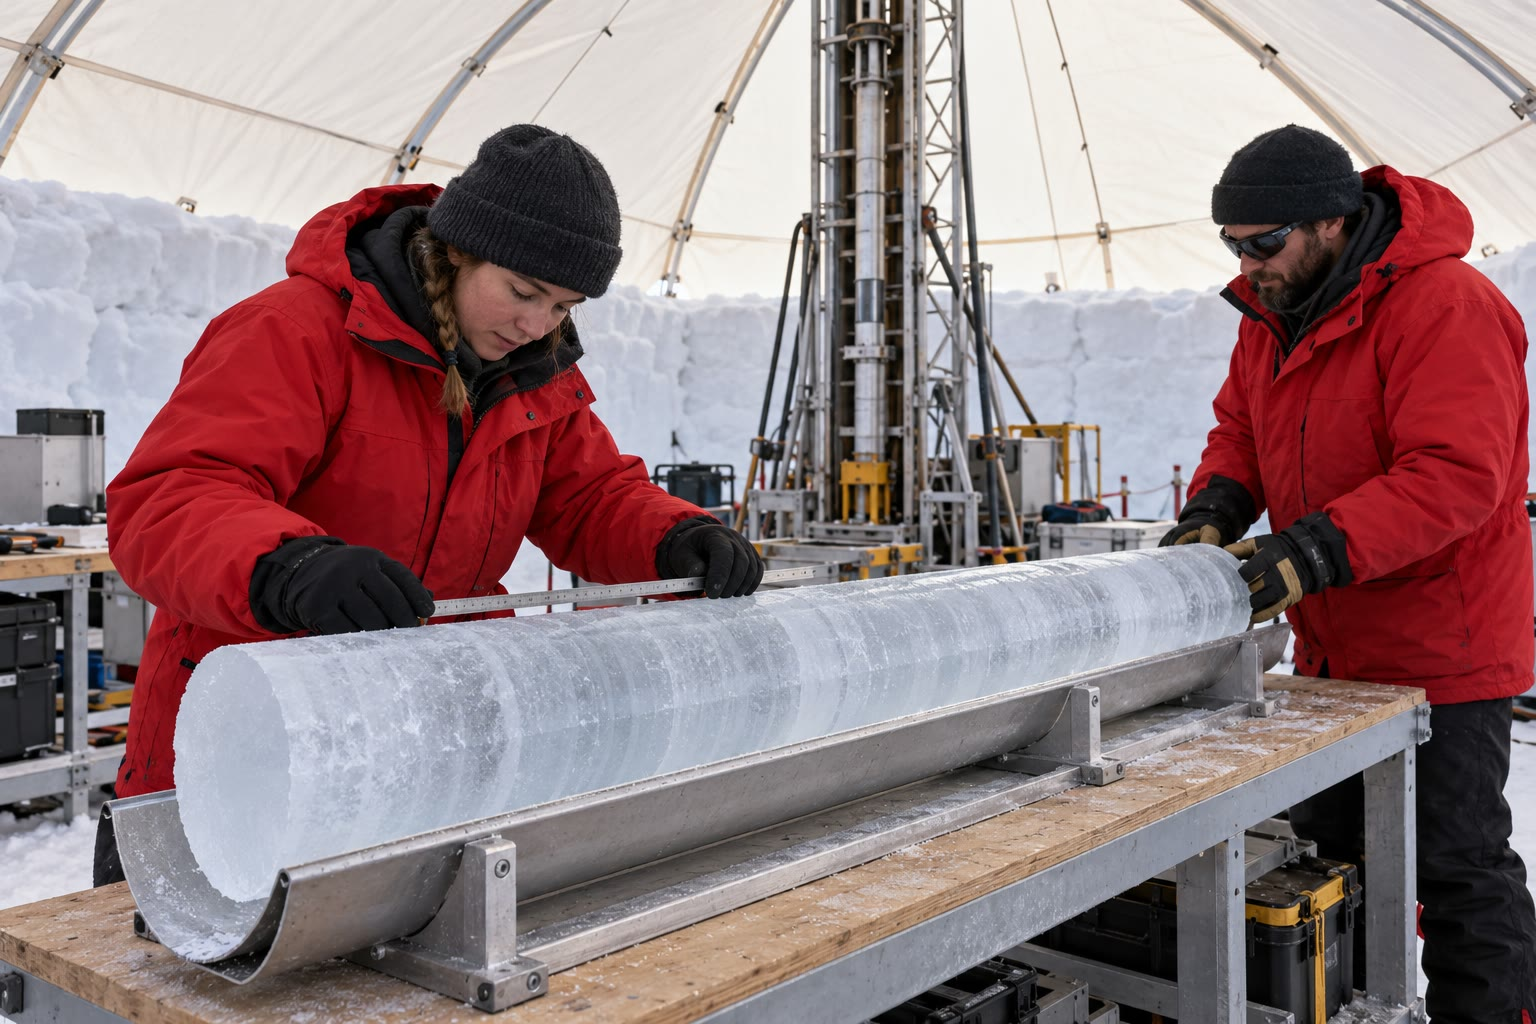
\includegraphics[width=\linewidth]{images/book5/ai/b3-ice-core-tent.jpg}

{\scriptsize Een ijskern wordt gemeten in een wieg in een boortent op een
ijskap, met de boortoren erachter. Door AI gegenereerde illustratie.}
\end{minipage}
\end{inthelab}

\section{Oefeningen}

\begin{exercise}[$\star$]\label{exo:b3:stable-isotopes:1}
Een calciet heeft $\delta^{18}\mathrm O = \qty{30.5}{\permil}$ en het water waaruit het groeide
heeft \qty{-2.1}{\permil}, beide op VSMOW. Bereken $\alpha$, $1000\ln\alpha$ en
$\Delta$. Hoe ver liggen de laatste twee uit elkaar?
\end{exercise}

\begin{exercise}[$\star$]\label{exo:b3:stable-isotopes:2}
Een kuststation op hoge breedte heeft een gemiddelde jaartemperatuur van
\qty{-25}{\celsius}. Voorspel met de verbanden uit het hoofdstuk voor zulke
stations de $\delta^{18}\mathrm O$, $\delta\mathrm D$ en het \omterm{def:b3:stable-isotopes:d-excess}{deuteriumoverschot} van
de neerslag.
\end{exercise}
% ledger: dansgaard64:effects

\begin{exercise}[$\star$]\label{exo:b3:stable-isotopes:3}
In een bekken hebben carbonaten $\delta^{13}\mathrm C = \qty{+1.0}{\permil}$ en organisch
materiaal \qty{-26.0}{\permil}. Met instromen bij \qty{-5}{\permil}, bereken
$f_{\mathrm{org}}$.
\end{exercise}
% ledger: planavsky22:forg

\begin{exercise}[$\star$]\label{exo:b3:stable-isotopes:4}
Een brachiopodenschelp heeft $\Delta_{47} = \qty{0.600}{\permil}$. Bij welke temperatuur
groeide hij, volgens de kalibratie van het hoofdstuk?
\end{exercise}
% ledger: isogeochem:d47

\begin{exercise}[$\star\star$]\label{exo:b3:stable-isotopes:5}
Waterdamp verlaat de oceaan met $\delta^{18}\mathrm O = \qty{-13}{\permil}$ en regent
uit met een constante $\alpha = 1.0100$. Welk deel ervan is over wanneer de
waterdamp \qty{-33}{\permil} bereikt? Wat is dan de $\delta^{18}\mathrm O$ van de
regen?
\end{exercise}
% ledger: white13c9:rayleigh

\begin{exercise}[$\star\star$]\label{exo:b3:stable-isotopes:6}
Sneeuw op \qty{-40}{\permil} wordt vergeleken met oceaanwater op 0. Bereken $\alpha$,
$1000\ln\alpha$, $1000(\alpha - 1)$ en $\Delta$ tussen beide. Welke van de
benaderingen van de propositie faalt, en met hoeveel?
\end{exercise}

\begin{exercise}[$\star\star$]\label{exo:b3:stable-isotopes:7}
Een foraminifeer heeft $\delta^{18}\mathrm O = \qty{+1.50}{\permil}$ VPDB en groeide in
water van \qty{0.00}{\permil} VSMOW. Bereken zijn groeitemperatuur met de
methode van het hoofdstuk, en hoeveel een fout van \qty{0.1}{\permil} in het water
de temperatuur verandert.
\end{exercise}
% ledger: isogeochem:ko97

\begin{exercise}[$\star\star$]\label{exo:b3:stable-isotopes:8}
De benthische stapel verandert met \qty{1.77}{\permil} van het heden tot het Laatste
Glaciale Maximum. Trek het ijsvolumeaandeel af dat in het hoofdstuk is berekend en
reken de rest om in een verandering van de diepwatertemperatuur, met de helling van de
calcietkalibratie nabij \qty{2}{\celsius}.
\end{exercise}
% ledger: data:lr04, white13c9:ice-volume, isogeochem:ko97

\begin{exercise}[$\star\star$]\label{exo:b3:stable-isotopes:9}
Een pyriet heeft $\delta^{34}\mathrm S = \qty{10.0}{\permil}$ en $\delta^{33}\mathrm S =
\qty{8.2}{\permil}$. Bereken $\Delta^{33}\mathrm S$. Wat zegt dit over de
atmosfeer toen de pyriet ontstond?
\end{exercise}
% ledger: white13c9:s-mif

\begin{exercise}[$\star\star\star$]\label{exo:b3:stable-isotopes:10}
Bij condensatie in een gesloten systeem blijven de waterdamp en al het gevormde
condensaat samen in evenwicht. Toon aan dat de waterdamp dan $R_v/R_{v,0} = 1/[f +
\alpha(1 - f)]$ heeft, en vergelijk dit met \omterm{prop:b3:stable-isotopes:rayleigh-distillation}{Rayleighdestillatie} voor $f = 0.2$ en
$\alpha = 1.01$.
\end{exercise}

\begin{exercise}[$\star\star\star$]\label{exo:b3:stable-isotopes:11}
Uit de schatting dat \qty{2000}{Gt} methaankoolstof bij
\qty{-60}{\permil} het uitwisselbare koolstof met \qty{-2.5}{\permil} verschuift,
bepaal de impliciete reservoirmassa, met $\delta_0 = 0$. Hoeveel organische koolstof bij
\qty{-25}{\permil} geeft met die massa dezelfde verschuiving? Vergelijk met het
gepubliceerde bereik.
\end{exercise}
% ledger: dickens11:petm

\begin{exercise}[$\star\star\star$]\label{exo:b3:stable-isotopes:12}
Toon aan dat, langs een afkoelingspad, $\mathrm d\delta_v/\mathrm dT = (\alpha - 1)(1000 +
\delta_v)\,\mathrm d\ln e_s/\mathrm dT$. Bereken bij \qty{-20}{\celsius}, waar de
waterdamp van het model van het hoofdstuk $\delta^{18}\mathrm O = \qty{-49.1}{\permil}$
heeft en de sublimatiecurve $\mathrm d\ln e_s/\mathrm dT =
\qty{0.0960}{K^{-1}}$ geeft. Bereken deze helling.
\end{exercise}
% ledger: gkinis14:alpha-ice, iapws:melt-subl

\section{Probleem: de reis van een regendruppel naar Dome Ilse}

\begin{problem}[{Weekendprobleem --- de isotopen van de sneeuw langs een
verzonnen traject, een paleotemperatuur en een koolstofexcursie}]\label{pb:b3:stable-isotopes:1}
Een luchtmassa verlaat de rand van een verzonnen ijskap bij \qty{0}{\celsius}
met waterdamp van $\delta^{18}\mathrm O = \qty{-20.0}{\permil}$ en $\delta\mathrm D =
\qty{-150}{\permil}$, en koelt bij constante druk af terwijl hij landinwaarts trekt.
Sneeuw vormt zich bij het station Coast bij \qty{-10}{\celsius}, bij Midway bij
\qty{-20}{\celsius} en bij Dome Ilse bij \qty{-30}{\celsius}, wanneer het deel van de
waterdamp dat over is $f = 0.425$, $0.169$ en $0.0622$ is. Gebruik de ijs--damp
fractioneringsfactoren van het hoofdstuk, constant over elk traject bij de waarde van
de middentemperatuur.
% ledger: gkinis14:alpha-ice, iapws:melt-subl, dansgaard64:effects, isogeochem:ko97, isogeochem:d47, white13c9:ice-volume, data:lr04, planavsky22:forg, dickens11:petm

\medskip\noindent\textbf{Deel I --- Destillatie.}
\begin{enumerate}
\item Bereken $\alpha^{18}$ en $\alpha^{\mathrm D}$ bij $-5$, $-10$, $-15$, $-20$,
$-25$ en \qty{-30}{\celsius} (vijf significante cijfers voor zuurstof, vier voor
deuterium).
\item Bereken de $\delta^{18}\mathrm O$ van de waterdamp bij aankomst in Coast.
\item Bereken die van de sneeuw van Coast.
\item Herhaal dit voor Midway (de trajectverhouding van $f$ is $0.169/0.425$).
\item Herhaal dit voor Dome Ilse.
\item Welk deel van de oorspronkelijke zuurstof-18 van de waterdamp zit nog in de lucht
bij Dome Ilse?
\end{enumerate}

\medskip\noindent\textbf{Deel II --- Temperatuur en deuterium.}
\begin{enumerate}[resume]
\item Bereken de helling van de $\delta^{18}\mathrm O$ van de sneeuw ten opzichte van de
condensatietemperatuur van Coast tot Dome Ilse.
\item Welke gemiddelde jaarlijkse oppervlaktetemperatuur zou het verband van de
Groenlandse stations aan de sneeuw van Dome Ilse toekennen? Waarom kan die
afwijken van \qty{-30}{\celsius}?
\item Bereken op dezelfde manier het $\delta\mathrm D$ van de sneeuw bij de drie stations.
\item Bereken hun \omterm{def:b3:stable-isotopes:d-excess}{deuteriumoverschot}. Hoe verandert dat landinwaarts?
\item Ligt de sneeuw van Dome Ilse op de meteorische waterlijn? Wat laat het model
weg wat echte sneeuwvorming wel bevat?
\end{enumerate}

\medskip\noindent\textbf{Deel III --- Een foraminifer voor de kust.} Een
sedimentkern voor de kust geeft benthische foraminiferen van \qty{3.25}{\permil}
VPDB bovenaan en \qty{5.02}{\permil} tijdens het Laatste Glaciale Maximum; het
bodemwater is vandaag \qty{0.00}{\permil} VSMOW.
\begin{enumerate}[resume]
\item Bereken de huidige temperatuur van het bodemwater met de
calcietkalibratie.
\item Bereken de glaciale temperatuur, aannemend dat het water onveranderd is. Is
het resultaat mogelijk?
\item Corrigeer het glaciale water voor een zeeniveaudaling van \qty{125}{m} en
herbereken. Wat is de glaciale afkoeling van het bodemwater?
\item Bereken het $\Delta_{47}$ dat bij beide temperaturen verwacht wordt en hun
verschil.
\item Waarom heeft de clumped-isotopenthermometer de samenstelling van
het water niet nodig?
\end{enumerate}

\medskip\noindent\textbf{Deel IV --- Een koolstofexcursie.} Dieper in de kern
worden carbonaten van \qty{+0.5}{\permil} onderbroken door een korte excursie van
\qty{-3.0}{\permil}.
\begin{enumerate}[resume]
\item Vóór de excursie, met $\delta_{\mathrm{in}} = \qty{-5}{\permil}$ en
$\Delta_B = \qty{-28}{\permil}$, bereken $f_{\mathrm{org}}$.
\item Neem het reservoir van oefening 11, \qty{46000}{Gt} bij 0. Hoeveel koolstof
heeft de excursie nodig als de bron methaan is bij \qty{-60}{\permil}?
\item En als het organische koolstof is bij \qty{-25}{\permil}?
\item En als het mantelkoolstof is bij \qty{-5}{\permil}?
\item Welke waarneming in dezelfde kern kan helpen om tussen de
bronnen te kiezen?
\item Geef het $\delta^{18}\mathrm O$ van de sneeuw die bij Dome Ilse valt.
\end{enumerate}
\end{problem}
